\documentclass[12pt,letterpaper,final]{report}
\usepackage[utf8]{inputenc}
\usepackage{amsmath}
\usepackage{amsfonts}
\usepackage{amssymb}
\usepackage{amsthm}
\renewcommand\qedsymbol{$\blacksquare$}
\usepackage{enumerate}
\usepackage{hyperref}
\usepackage{pdfpages}
\usepackage{graphics}
\usepackage{graphicx}
\usepackage{tikz}
\usepackage{tikz-qtree}
\usetikzlibrary{automata,arrows, arrows.meta, positioning}
\usepackage[
  backend=biber,
  style=authoryear,
  sorting=nyt          % sort by name, year, title
]{biblatex}
\addbibresource{references.bib}

% \author{Marius Zimand}
\author{Jonathan Llovet}

\begin{document}

\fbox{
	\vbox{
		\begin{flushleft}
			Jonathan Llovet \\  % authors' names
			COSC 417 \\  %class
			2026-02-19, 11:59 PM (EST) \\  % date
		\end{flushleft}
		\center{\Large{\textbf{Assignment 2}}}
		%\end{mdframed}
	} % end vbox
} % end fbox
\vline

Do (or at least sketch the solutions) without turning in anything the following exercises from the textbook: 1.4 (a-d), 1.5 (a-d), 1.6(a-d), 1.7(a-d).

\medskip

{\bf Problem 1.}  The formal description of a DFA $M$ is $(\{q_1, q_2, q_3, q_4, q_5\}, \{u,d\}, \delta , q_3, \{q_3\})$, where  $\delta$ is given by the following table. Draw the state diagram (i.e.\,  the graph representation) of this machine.
\smallskip

\begin{tabular}{|l|ll|}
	\hline
	       & $u$    & $d$   \\
	\hline
	$q_1$  & $q_1$  & $q_2$ \\
	$q_2 $ & $q_1$  & $q_3$ \\
	$q_3$  & $q_2 $ & $q_4$ \\
	$q_4$  & $q_3$  & $q_5$ \\
	$q_5$  & $q_4$  & $q_5$ \\
	\hline
\end{tabular}
\smallskip

\begin{center}
	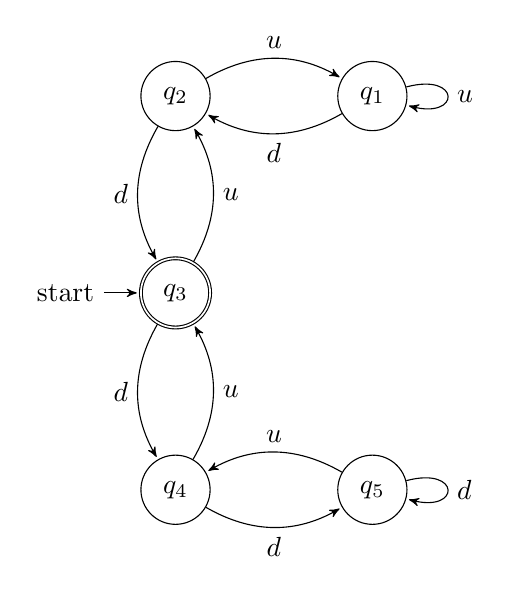
\begin{tikzpicture}[>=stealth',shorten >=1pt,auto,node distance=2.5cm]

		\node[initial, state, accepting] (3) {$q_{3}$};
		\node[state] (2) [above of=3] {$q_{2}$};
		\node[state] (1) [right of=2] {$q_{1}$};
		\node[state] (4) [below of=3] {$q_{4}$};
		\node[state] (5) [right of=4] {$q_{5}$};

		\path[->]
		(1) edge [loop right] node {$u$} (1)
		(1) edge [bend left] node[below] {$d$} (2)

		(2) edge [bend left] node[above] {$u$} (1)
		(2) edge [bend right] node[left] {$d$} (3)

		(3) edge [bend right] node[right] {$u$} (2)
		(3) edge [bend right] node[left] {$d$} (4)

		(4) edge [bend right] node[right] {$u$} (3)
		(4) edge [bend right] node[below] {$d$} (5)

		(5) edge [bend right] node[above] {$u$} (4)
		(5) edge [loop right] node {$d$} (5)
		;
	\end{tikzpicture}
\end{center}

\medskip

Show the computation done by this machine on input $uddu$ (i.e., the sequence of states it enters; see Example 1.17 in the textbook).

The sequence of states the DFA above enters when computing the string $uddu$ is
$q_3, q_2, q_3, q_4, q_3$

\medskip

{\bf Problem 2.}	 	Give the state diagram of DFAs with the specified number of states (or less) for each of the following languages over the alphabet $\{0,1\}$. For each of the three DFA briefly and convincingly explain (give a ``common sense" explanation, I don't require a formal proof) why they accept the specified language.

\begin{enumerate}

	\item[a.]	$\{w \mid w \mbox{ begins with a $1$ and ends with a $0$}\}$, DFA with $4$ states.  Show the computation (i.e., the sequence of states it enters; see Example 1.17 in the textbook) made by your DFA on input 10010 and on input 110011.

	      \begin{center}
		      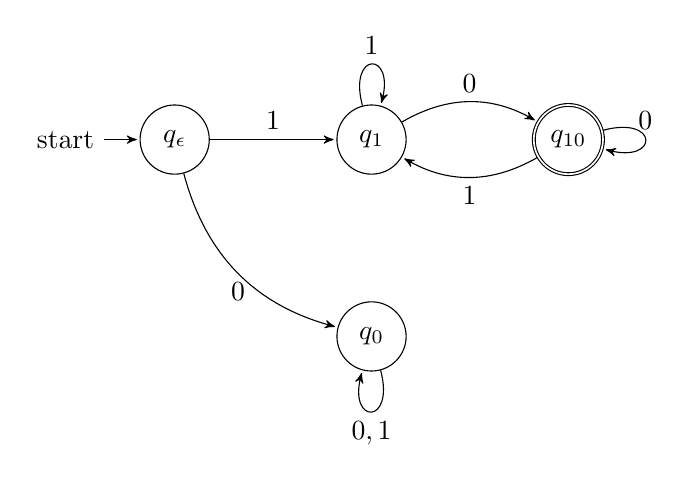
\begin{tikzpicture}[>=stealth',shorten >=1pt,auto,node distance=2.5cm]

			      \node[initial, state] (e) {$q_{\epsilon}$};
			      \node[state] (1) [right of=e] {$q_{1}$};
			      \node[state, accepting] (10) [right of=1] {$q_{10}$};
			      \node[state] (0) [below of=1] {$q_{0}$};

			      \path[->]
			      (e) edge [bend right] node[below] {$0$} (0)
			      (e) edge node[above] {$1$} (1)
			      (1) edge [loop above] node[above] {$1$} (1)
			      (1) edge [bend left] node[above] {$0$} (10)

			      (10) edge [loop right] node[above] {$0$} (10)
			      (10) edge [bend left] node[below] {$1$} (1)

			      (0) edge [loop below] node[below] {$0,1$} (0)
			      ;
		      \end{tikzpicture}
	      \end{center}

	      {\bf Input:} $10010$, {\bf States:} $q_{\epsilon}, q_{1}, q_{10}, q_{10}, q_{1}, q_{10}$

	      {\bf Input:} $110011$, {\bf States:} $q_{\epsilon}, q_{1}, q_{1}, q_{10}, q_{10}, q_{1}, q_{1}$

	      {\bf How it works:} This DFA has two branches to go down. The strings starting with $0$ will fall into the sink on the bottom branch going to $q_0$, while strings starting with $1$ will be routed along the top path to $q_1$ and potentially to the accepting state $q_{10}$. If the string has a sequence of one or more $0$'s at the end, it will go to the far right. If a $1$ comes up, then it will go back to $q_1$ until another $0$ is encountered.

	      \pagebreak
	\item[b.]	$\{w \mid w \mbox{ starts with $0$ and has odd length, or starts with $1$ and has even length}\}$, DFA with $3$ states. Show the computation (i.e., the sequence of states) made by your DFA on input 100101 and on input 11001.


	      \begin{center}
		      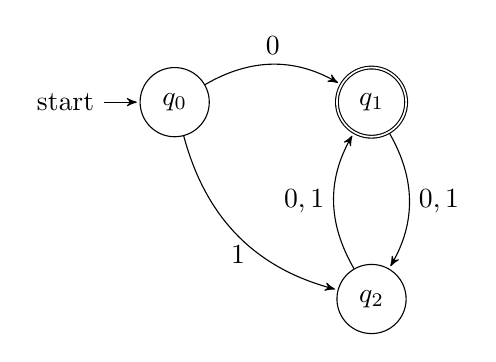
\begin{tikzpicture}[>=stealth',shorten >=1pt,auto,node distance=2.5cm]

			      \node[initial, state] (0) {$q_{0}$};
			      \node[state, accepting] (1) [right of=0] {$q_{1}$};
			      \node[state] (2) [below of=1] {$q_{2}$};

			      \path[->]
			      (0) edge [bend left] node[above] {$0$} (1)
			      (0) edge [bend right] node[below] {$1$} (2)

			      (1) edge [bend left] node[right] {$0,1$} (2)

			      (2) edge [bend left] node[left] {$0,1$} (1)
			      ;
		      \end{tikzpicture}
	      \end{center}

	      {\bf Input:} $100101$, {\bf States:} $q_0, q_2, q_1, q_2, q_1, q_2, q_1$

	      {\bf Input:} $11001$, {\bf States:} $q_0, q_2, q_1, q_2, q_1, q_2$

	      {\bf How it works:} If a string starts with $0$, at first it will be in an accepting state because the string has one letter and is hence of odd length. If there are more letters, then it will cycle back and forth between $q_1$ and $q_2$, where $q_2$ will represent that the string is of even length. However, if a string starts with $1$, then $q_2$ represents the scenario where the string is of odd length (and hence not accepting). Then, if the string starting with 1 has subsequent letters, the state will alternate similarly between $q_2$ (accepting) to $q_1$.

	      It's notable that there is an inversion of the parity represented by states $q_1$ and $q_2$ depending on what the starting value of the string is, which makes this a little subtle to interpret.

	      \pagebreak

	\item[c.]	$\{w \mid w \mbox{ does not contain the string 110}\}$, DFA  with $4$ states. Show the computation (i.e., the sequence of states) made by your DFA on input 1001101 and on input 1001.

	      \begin{center}
		      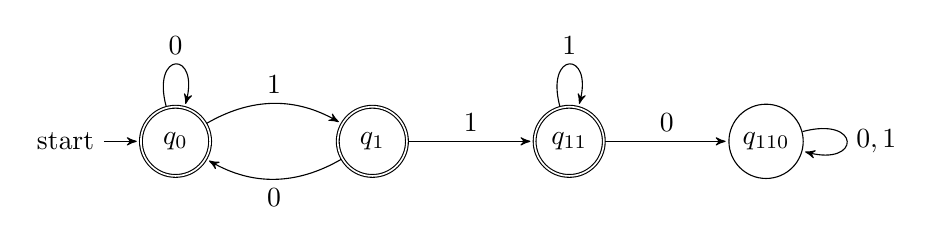
\begin{tikzpicture}[>=stealth',shorten >=1pt,auto,node distance=2.5cm]

			      \node[initial, state, accepting] (0) {$q_{0}$};
			      \node[state, accepting] (1) [right of=0] {$q_{1}$};
			      \node[state, accepting] (11) [right of=1] {$q_{11}$};
			      \node[state] (110) [right of=11] {$q_{110}$};

			      \path[->]
			      (0) edge [loop above] node[above] {$0$} (0)
			      (0) edge [bend left] node[above] {$1$} (1)

			      (1) edge [bend left] node[below] {$0$} (0)
			      (1) edge node[above] {$1$} (11)

			      (11) edge [loop above] node[above] {$1$} (11)
			      (11) edge node[above] {$0$} (110)

			      (110) edge [loop right] node[right] {$0,1$} (110)
			      ;
		      \end{tikzpicture}
	      \end{center}

	      {\bf Input:} $1001101$, {\bf States:} $q_0, q_1, q_0, q_0, q_1, q_{11}, q_{110}, q_{110}$

	      {\bf Input:} $1001$, {\bf States:} $q_0, q_1, q_0, q_0, q_1$

	      {\bf How it works:} This DFA starts in an accepting state and allows the input to go through more restrictive states as it gets closer and closer to the unaccepting state - that is, until it reaches the point of no return, after which it falls into a sink and will not be accepted. If there are only $0$'s, the DFA will loop on $q_0$. If there are $1$'s and $0$'s alternating, then the state will alternate between $q_0$ and $q_1$. Once there are two consecutive $1$'s though, we are in a bit of a trap. From then on, the string can only be accepted if all of the subsequent values are $1$, since any subsequent $0$ would allow the illegal substring $110$. So, once there are multiple $1$'s, all the remaining letters will have to be $1$'s for the DFA to accept the string, otherwise it will reject it.

\end{enumerate}

\pagebreak

{\bf Problem 3.}	 Give NFAs (in the form of state diagrams) with the specified number of states recognizing each the following languages. The alphabet is $\Sigma =\{0,1\}$. As above, explain why your NFAs accept the corresponding language.
\begin{enumerate}
	\item[a.]	$\{w \mid w \mbox{ ends with 00}\}$ with 3 states. Pick one input string that is in the language and one input string that is not in the language and show the two trees of computation possibilities made by your NFA on the two strings (as we did in class, see also Figure 1.29 in the textbook).

	      \begin{center}
		      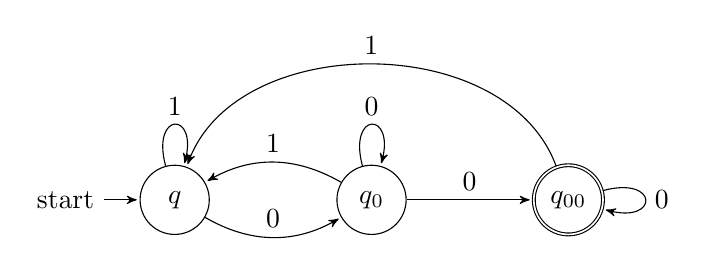
\begin{tikzpicture}[>=stealth',shorten >=1pt,auto,node distance=2.5cm]

			      \node[initial, state] (q) {$q$};
			      \node[state] (0) [right of=q] {$q_{0}$};
			      \node[state, accepting] (00) [right of=0] {$q_{00}$};

			      \path[->]
			      (q) edge [loop above] node[above] {$1$} (q)
			      (q) edge [bend right] node[above] {$0$} (0)

			      (0) edge [loop above] node[above] {$0$} (0)
			      (0) edge [bend right] node[above] {$1$} (q)
			      (0) edge node[above] {$0$} (00)

			      (00) edge [loop right] node[right] {$0$} (0)
			      (00) edge [bend right=70] node[above] {$1$} (q)
			      ;
		      \end{tikzpicture}
	      \end{center}

	      \begin{center}

		      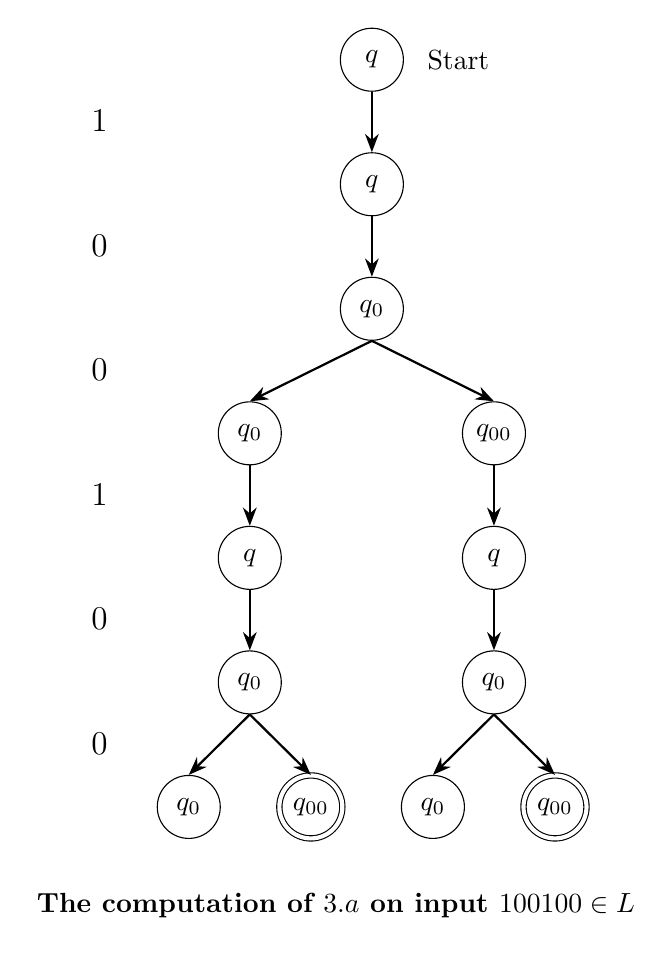
\begin{tikzpicture}[
				      % Node styles
				      state/.style={
						      circle, draw, minimum size=8mm, inner sep=0pt,
						      font=\normalsize,
					      },
				      accept state/.style={
						      state, double, double distance=1.5pt,
					      },
				      % Edge/arrow style — applied globally to the tree
				      edge from parent/.style={
						      draw, thick, ->, >=Stealth,
					      },
				      % Increase level distance (vertical spacing between levels)
				      level distance=45pt,
				      % Increase sibling distance (horizontal spacing)
				      sibling distance=20pt,
			      ]
			      % \begin{noindent}
            \Tree
            [.\node[state](root1){$q$};
              [.\node[state]{$q$};
                [.\node[state]{$q_0$};
                  [.\node[state]{$q_0$};
                    [.\node[state]{$q$};
                      [.\node[state]{$q_0$};
                        [.\node[state]{$q_0$};]
                        [.\node[accept state]{$q_{00}$};]
                      ]
                    ]
                  ]
                  [.\node[state]{$q_{00}$};
                    [.\node[state]{$q$};
                      [.\node[state]{$q_0$};
                        [.\node[state]{$q_0$};]
                        [.\node[accept state]{$q_{00}$};]
                      ]
                    ]
                  ]
                ]
              ]
            ]
            \node[right=5pt of root1] {Start};
            % \end{noindent}

			      % --- Symbol labels on the left side ---
			      % We position these relative to the tree's bounding box.
			      % Adjust x-coordinates as needed for your tree width.
			      \begin{scope}[symbol label/.style={font=\large, anchor=east}]
				      % Grab the root's y-coordinate as reference; levels are spaced by 55pt
				      \path (current bounding box.north west) +(-0.5, 0) coordinate (labelanchor);

				      \foreach \sym/\i in {1/1, 0/2, 0/3, 1/4, 0/5, 0/6} {
						      \node[symbol label] at ([yshift={-(\i-0.25)*45pt}] labelanchor) {\sym};
					      }
			      \end{scope}

			      % --- Caption ---
			      \node[font=\bfseries, anchor=north] at
			      ([yshift=-15pt] current bounding box.south)
			      {The computation of $3.a$ on input $100100 \in L$};

		      \end{tikzpicture}
	      \end{center}

	      \begin{center}

		      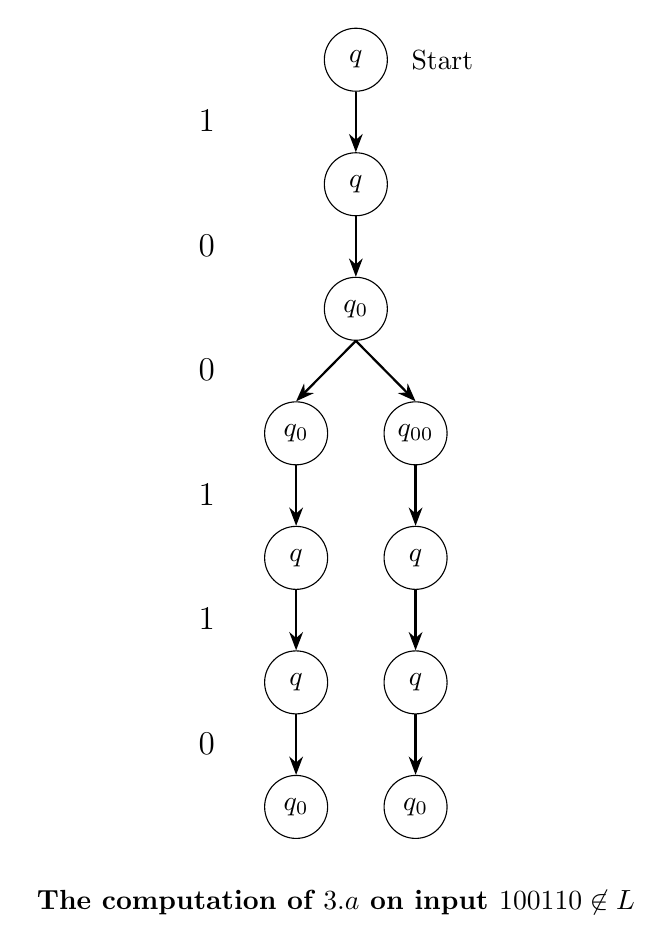
\begin{tikzpicture}[
				      % Node styles
				      state/.style={
						      circle, draw, minimum size=8mm, inner sep=0pt,
						      font=\normalsize,
					      },
				      accept state/.style={
						      state, double, double distance=1.5pt,
					      },
				      % Edge/arrow style — applied globally to the tree
				      edge from parent/.style={
						      draw, thick, ->, >=Stealth,
					      },
				      % Increase level distance (vertical spacing between levels)
				      level distance=45pt,
				      % Increase sibling distance (horizontal spacing)
				      sibling distance=20pt,
			      ]
			      % \begin{noindent}
            \Tree
            [.\node[state](root2){$q$};
              [.\node[state]{$q$};
                [.\node[state]{$q_0$};
                  [.\node[state]{$q_0$};
                    [.\node[state]{$q$};
                      [.\node[state]{$q$};
                        [.\node[state]{$q_0$};]
                      ]
                    ]
                  ]
                  [.\node[state]{$q_{00}$};
                    [.\node[state]{$q$};
                      [.\node[state]{$q$};
                        [.\node[state]{$q_0$};]
                      ]
                    ]
                  ]
                ]
              ]
            ]
            \node[right=5pt of root2] {Start};
            % \end{noindent}

			      % --- Symbol labels on the left side ---
			      % We position these relative to the tree's bounding box.
			      % Adjust x-coordinates as needed for your tree width.
			      \begin{scope}[symbol label/.style={font=\large, anchor=east}]
				      % Grab the root's y-coordinate as reference; levels are spaced by 55pt
				      \path (current bounding box.north west) +(-0.5, 0) coordinate (labelanchor);

				      \foreach \sym/\i in {1/1, 0/2, 0/3, 1/4, 1/5, 0/6} {
						      \node[symbol label] at ([yshift={-(\i-0.25)*45pt}] labelanchor) {\sym};
					      }
			      \end{scope}

			      % --- Caption ---
			      \node[font=\bfseries, anchor=north] at
			      ([yshift=-15pt] current bounding box.south)
			      {The computation of $3.a$ on input $100110 \not\in L$};

		      \end{tikzpicture}
	      \end{center}

	      {\bf How it works:} This NFA works by accumulating 0s moving from state $q$ to state $q_0$ to state $q_{00}$. If we have encountered two $0$ values in a row, that will be sufficient for the state $q_{00}$ to be reached. Because the last two values need to be $0$'s, if at any point the automaton encounters a $1$, the state transitions back to the starting state. There is a redundant transition looping from $q_0$ to itself, which allows the nondeterministic character of the NFA to appear more clearly. A simplified DFA could be built to perform the same computation where the states and transitions would be the same, with the omission of the loop on $q_0$.

	      \pagebreak
	\item[b.]	$\{w \mid w \mbox{ contains the substring 0101}\}$ with 5 states. Pick one input string that is in the language and one input string that is not in the language and show the two trees of computation possibilities made by your NFA on the two strings.
        \begin{center}
		      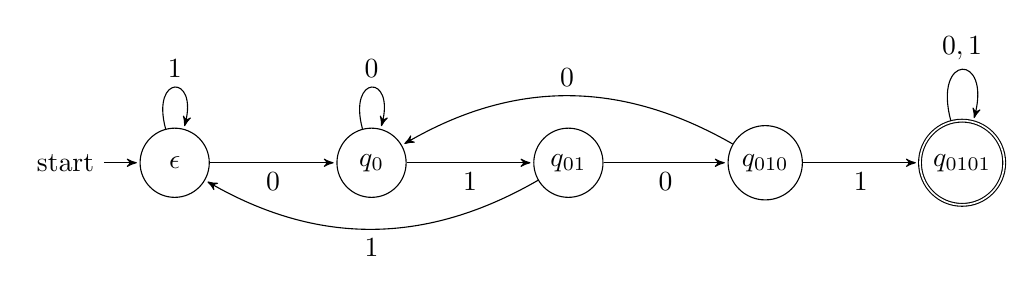
\begin{tikzpicture}[>=stealth',shorten >=1pt,auto,node distance=2.5cm]

			      \node[initial, state] (e) {$\epsilon$};
			      \node[state] (0) [right of=e] {$q_{0}$};
			      \node[state] (01) [right of=0] {$q_{01}$};
			      \node[state] (010) [right of=01] {$q_{010}$};
			      \node[state, accepting] (0101) [right of=010] {$q_{0101}$};

			      \path[->]

			      (e) edge [loop above] node[above] {$1$} (e)
			      (e) edge node[below] {$0$} (0)
			      
            (0) edge [loop above] node[above] {$0$} (0)
            (0) edge node[below] {$1$} (01)
			      % (q) edge [bend right] node[above] {$0$} (0)
            (01) edge node[below] {$0$} (010)
            (01) edge [bend left] node[below] {$1$} (e)
            
            (010) edge node[below] {$1$} (0101)
            (010) edge [bend right] node[above] {$0$} (0)
            
			      (0101) edge [loop above] node[above] {$0,1$} (0101)
			      % (00) edge [bend right=70] node[above] {$1$} (q)
			      ;
		      \end{tikzpicture}
	      \end{center}

	      \begin{center}

		      \begin{tikzpicture}[
				      % Node styles
				      state/.style={
						      circle, draw, minimum size=8mm, inner sep=0pt,
						      font=\normalsize,
					      },
				      accept state/.style={
						      state, double, double distance=1.5pt,
					      },
				      % Edge/arrow style — applied globally to the tree
				      edge from parent/.style={
						      draw, thick, ->, >=Stealth,
					      },
				      % Increase level distance (vertical spacing between levels)
				      level distance=45pt,
				      % Increase sibling distance (horizontal spacing)
				      sibling distance=20pt,
			      ]
			      % \begin{noindent}
            \Tree
            [.\node[state](root1){$\epsilon$};
              [.\node[state]{$\epsilon$};
                [.\node[state]{$q_0$};
                  [.\node[state]{$q_0$};
                    [.\node[state]{$q_{01}$};
                      [.\node[state]{$q_{010}$};
                        [.\node[accept state]{$q_{0101}$};]
                      ]
                    ]
                  ]
                ]
              ]
            ]
            \node[right=5pt of root1] {Start};
            % \end{noindent}

			      % --- Symbol labels on the left side ---
			      % We position these relative to the tree's bounding box.
			      % Adjust x-coordinates as needed for your tree width.
			      \begin{scope}[symbol label/.style={font=\large, anchor=east}]
				      % Grab the root's y-coordinate as reference; levels are spaced by 55pt
				      \path (current bounding box.north west) +(-0.5, 0) coordinate (labelanchor);

				      \foreach \sym/\i in {1/1, 0/2, 0/3, 1/4, 0/5, 1/6} {
						      \node[symbol label] at ([yshift={-(\i-0.25)*45pt}] labelanchor) {\sym};
					      }
			      \end{scope}

			      % --- Caption ---
			      \node[font=\bfseries, anchor=north] at
			      ([yshift=-15pt] current bounding box.south)
			      {The computation of $3.b$ on input $100101 \in L$};

		      \end{tikzpicture}
	      \end{center}

	      \begin{center}

		      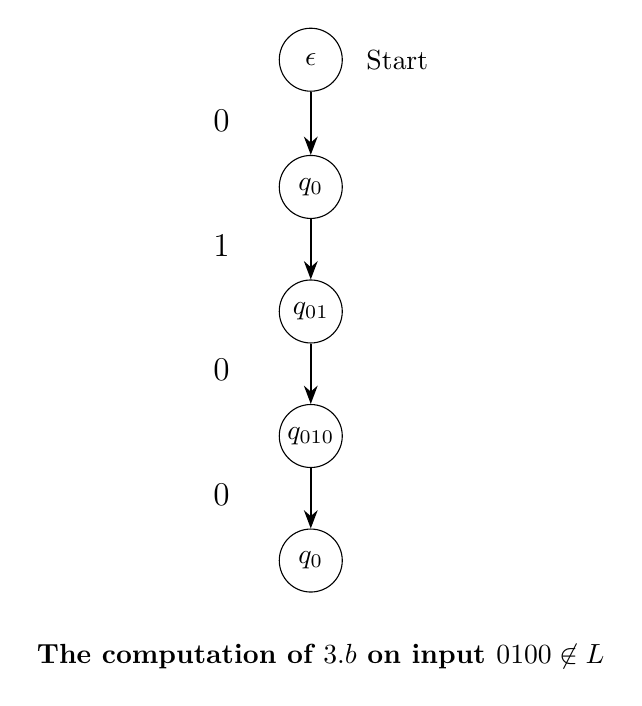
\begin{tikzpicture}[
				      % Node styles
				      state/.style={
						      circle, draw, minimum size=8mm, inner sep=0pt,
						      font=\normalsize,
					      },
				      accept state/.style={
						      state, double, double distance=1.5pt,
					      },
				      % Edge/arrow style — applied globally to the tree
				      edge from parent/.style={
						      draw, thick, ->, >=Stealth,
					      },
				      % Increase level distance (vertical spacing between levels)
				      level distance=45pt,
				      % Increase sibling distance (horizontal spacing)
				      sibling distance=20pt,
			      ]
			      % \begin{noindent}
            \Tree
            [.\node[state](root1){$\epsilon$};
              [.\node[state]{$q_0$};
                [.\node[state]{$q_{01}$};
                  [.\node[state]{$q_{010}$};
                    [.\node[state]{$q_{0}$};]
                  ]
                ]
              ]
            ]
            \node[right=5pt of root1] {Start};
            % \end{noindent}

			      % --- Symbol labels on the left side ---
			      % We position these relative to the tree's bounding box.
			      % Adjust x-coordinates as needed for your tree width.
			      \begin{scope}[symbol label/.style={font=\large, anchor=east}]
				      % Grab the root's y-coordinate as reference; levels are spaced by 55pt
				      \path (current bounding box.north west) +(-0.5, 0) coordinate (labelanchor);

				      \foreach \sym/\i in {0/1, 1/2, 0/3, 0/4} {
						      \node[symbol label] at ([yshift={-(\i-0.25)*45pt}] labelanchor) {\sym};
					      }
			      \end{scope}

			      % --- Caption ---
			      \node[font=\bfseries, anchor=north] at
			      ([yshift=-15pt] current bounding box.south)
			      {The computation of $3.b$ on input $0100 \not \in L$};

		      \end{tikzpicture}
	      \end{center}

	      {\bf How it works:} This NFA is actually also a DFA. The computation is straightforward in both cases, where the input is in the language and when it is not. The strategy as in several of the other cases is to accumulate letters of the substring, with transitions to go back to earlier states in cases where the opposite letter than is required is provided (viz. in states $q_{01}$ and $q_{010}$, the state gets knocked back to an earlier one if anything other than the next required letter to build up the substring). This is precisely what occurs with the input $0100$. It is at the penultimate state and then is knocked back to $q_0$, without sufficient input to accumulate the required substring again before the end of the input.

\end{enumerate}

\pagebreak

{\bf Problem 4.}	 For any string $w_1 w_2 \ldots w_n$, the reverse $w^R$  is the string $w$ in reverse order $w_n  \ldots w_2 w_1$.   For a language $A$, let $A^R = \{ w^R \mid w \mbox{ is in }A\}$ (in other words, $A^R$ consists of all the reverses of the strings in $A$).  Prove that if $A$ is regular, then $A^R$  is also regular. In your proof you have to  show how to convert a finite automaton for $A$ into a finite automaton for $A^R$.  Other arguments are possible, but will not give you the extra credit. (Note: Take care, an FA, whether deterministic or nondeterministic, has a single starting state).

{\bf Proof:} Assume that a language $A$ is regular. Because $A$ is regular, there is a finite automaton that recognizes $A$. Let it be called $M_A$. We will prove that the language $A^R$, which is composed of the reverse of each of the strings in $A$, is a regular language by transforming the finite automaton $M_A$ into a finite automaton $M_{A^R}$, since if there is a finite automaton $M_{A^R}$ that recognizes $A^R$, then $A^R$ is regular.

Because $M_A$ is a finite automaton, it is defined as a tuple
\[
  \big(Q, \Sigma, \delta, q_0, F \big)
\]
or
\[
  \big( \{q_0, q_1, \ldots, q_n\}, \{0, 1\}, \delta, q_0, \{q_{f0}, q_{f1},\ldots, q_{fn}\} \big)
\]
where $\delta$ is a transition function that maps states from $Q$ to each other according to the current input letter $w_k \in \Sigma$ from a string ${w_1}{w_2}{w_k}\ldots{w_m}$ provided to the state:
\[
  \delta(q_i, w_k) \to q_j \text{, where } i, j \in {0,
  \ldots, n}.
\]
Proceeding from the starting state $q_0$, each string $w \in A$ will induce a path from the starting state $q_0$ to some accepting state $q_f \in F$. To produce the reverse of a given path, we must begin on that formerly accepting state $q_f$, and then we must proceed backwards along each transition that was traversed until we exhaust the reversed input string and are back on the former starting state $q_0$. For a single path this is non-problematic and straightforward. However, in order to handle every string in the language A, we will have an obstacle. Namely, as mentioned above, every automaton has only one starting state. So, we cannot construct the automaton $M_{A^R}$ merely by replacing $q_0$ with $q_f$, since that would not recognize all strings in $A^R$. Rather, we will have to take advantage of the equivalence of NFA's and DFA's.

Let us construct an NFA whose states are $Q_A \cup q_{\epsilon}$, where $q_{\epsilon}$ will serve as the new starting state. From $q_{\epsilon}$, let there be an $\epsilon$ transition (empty string transition) to every state that was formerly an accepting state. Then, for each mapping in the transition function $\delta$, let the states be switched, so that we will proceed backwards and nondeterministically from $q_{\epsilon}$ immediately to each state $q_f \in F_A$, through the intermediate states in reverse order and ultimately back to the original $q_0$ from $A$.

Adapting the definition of $A$ from above, $A^R$ is defined as:

\[
  \big(Q \cup \{q_{\epsilon}\}, \Sigma, \delta_{A^R}, q_{\epsilon}, F_{A^R} \big)
\]
that is,
\[
  \big( \{q_0, q_1, \ldots, q_n\} \cup \{q_{\epsilon}\}, \{0, 1\}, \delta_{A^R}, q_{\epsilon}, \{q_0\} \big)
\]
where $\delta_{A^R}$ is the following, modified from $\delta_{A}$,
\[
\begin{array}{lll}
  \forall q_f \in F_A, \delta(q_{\epsilon}, \epsilon) &\to q_f \\
  \cup \\
  \delta(q_j, w_k) &\to q_i \text{, where } i, j \in {0,
  \ldots, n}.
\end{array}
\]

That is, from our new dummy starting state $q_{\epsilon}$, there is an epsilon transition to each of the accepting states from $A$. Then, the source and target states are reversed for each mapping in the original transition function $\delta_A$.

Because this NFA proceeds nondeterministically from each of the accepting states of $A$ back through each of the paths corresponding to the reversed strings $w^R \in A^R$, this NFA $M_{A^R}$ recognizes $A^R$. Because of the equivalence of NFA's and DFA's, it is possible to transform this NFA into a DFA. Critically, though, because we have shown how to construct a finite automaton $M_{A^R}$ that recognizes $A^R$, we have demonstrated that $A^R$ is a regular language. Therefore, $A$ is regular $\implies$ $A^R$ is regular.

\qed

\end{document}
